\chapter{DATA SETS AND SAMPLE DEFINITIONS}
\label{chap:EventSelect}

\section{Data Samples}

As already mentioned, this analysis was performed using 35.9 \fbinv collected with the CMS detector in 2016. More specifically, the data sets listed in Table~\ref{tab:datasets} were used. These correspond to the reprocessing of the data that took place in February 2017 to include improved calibrations and performance corrections. The relevant ``golden JSON" file was used to specify which events passed all of the offline CMS data quality monitoring requirements: \\
Cert$\_$271036-284044$\_$13TeV$\_$23Sep2016ReReco$\_$Collisions16$\_$JSON.txt

\begin{table}[ht]
\caption{DATA SAMPLES}
\label{tab:datasets}
\begin{center}
\begin{tabular}{|>{\centering\arraybackslash}m{0.9\linewidth}|}
\hline
%\hline
%\textbf{Data sets} \\
\hline
/DoubleEG/Run2016B-03Feb2017$\_$ver2-v2/MINIAOD \\
/DoubleEG/Run2016C-03Feb2017-v1/MINIAOD \\
/DoubleEG/Run2016D-03Feb2017-v1/MINIAOD \\
/DoubleEG/Run2016E-03Feb2017-v1/MINIAOD \\
/DoubleEG/Run2016F-03Feb2017-v1/MINIAOD \\
/DoubleEG/Run2016G-03Feb2017-v1/MINIAOD \\
/DoubleEG/Run2016H-03Feb2017$\_$ver2-v1/MINIAOD \\
/DoubleEG/Run2016H-03Feb2017$\_$ver3-v1/MINIAOD \\      
\hline
\hline
\end{tabular}
 \justify{List of data samples used in this analysis.}
\end{center}
\end{table}

\section{MC Samples}
\label{sec:MC}
Monte Carlo (MC) simulations are used for several purposes in this analysis. Simulations
of the signal processes are used to determine signal efficiencies, and
background process simulations are used for validation of the analysis performance
and to model the contribution from $Z\gamma\gamma\rightarrow\nu\nu\gamma\gamma$
events. The full list of MC samples for this analysis is shown in Table~\ref{tab:MC}.
The details of the signal simulation will be described in more detail in Section~\ref{sec:SimplifiedModels}. 

\begin{table}[ht]
\caption{MC SAMPLES FOR SIGNAL AND BACKGROUND}
\label{tab:MC}
\begin{center}
\begin{tabular}{|>{\centering\arraybackslash}m{0.9\linewidth}|}
\hline
\hline
\bf{SUSY Signal Samples}   \\         
\hline                                                                                         
\small{/SMS-T5Wg$\_$TuneCUETP8M1$\_$13TeV-madgraphMLM-pythia8/
          RunIISpring16MiniAODv2-PUSpring16Fast$\_$80X$\_$mcRun2$\_$
          asymptotic$\_$2016$\_$miniAODv2$\_$v0-v1/MINIAODSIM }\\
\hline
\small{/SMS-T5Wg$\_$mGo2150To2500$\_$TuneCUETP8M1$\_$13TeV-madgraphMLM-pythia8/
          RunIISpring16MiniAODv2-PUSpring16Fast$\_$80X$\_$mcRun2$\_$ 
          asymptotic$\_$2016$\_$miniAODv2$\_$v0-v1/MINIAODSIM }\\
\hline
\small{/SMS-T6Wg$\_$TuneCUETP8M1$\_$13TeV-madgraphMLM-pythia8/ 
 		     RunIISpring16MiniAODv2-PUSpring16Fast$\_$80X$\_$mcRun2$\_$ 
		     asymptotic$\_$2016$\_$miniAODv2$\_$v0-v1/MINIAODSIM }\\
\hline
\small{/SMS-T6Wg$\_$TuneCUETP8M1$\_$13TeV-madgraphMLM-pythia8/ 
          RunIISpring16MiniAODv2-PUSpring16Fast$\_$80X$\_$mcRun2$\_$ 
          asymptotic$\_$2016$\_$miniAODv2$\_$v0-v1/MINIAODSIM }\\
\hline                                               
\bf{Background MC Samples} \\ 
\hline                                                                                      
\small{/GJet$\_$Pt-40toInf$\_$DoubleEMEnriched$\_$MGG-80toInf$\_$TuneCUETP8M1$\_$13TeV$\_$Pythia8/ 
%\footnotesize{/GJet$\_$Pt-40toInf$\_$DoubleEMEnriched$\_$MGG-80toInf$\_$/
RunIISummer16MiniAODv2-PUMoriond17$\_$80X$\_$mcRun2$\_$ 
asymptotic$\_$2016$\_$TrancheIV$\_$v6-v1/MINIAODSIM} \\
\hline
\small{/ZGGToNuNuGG$\_$5f$\_$TuneCUETP8M1$\_$13TeV-amcatnlo-pythia8/
RunIISummer16MiniAODv2-PUMoriond17$\_$80X$\_$mcRun2$\_$
asymptotic$\_$2016$\_$TrancheIV$\_$v6-v1/MINIAODSIM }\\
\hline
\small{/DYJetsToLL$\_$M-50$\_$TuneCUETP8M1$\_$13TeV-madgraphMLM-pythia8/ 
RunIISpring16MiniAODv2-PUSpring16$\_$80X$\_$mcRun2$\_$
asymptotic$\_$2016$\_$miniAODv2$\_$v0$\_$ext1-v1/MINIAODSIM }\\                     
\hline
\hline
\end{tabular}
 \justify{List of MC samples used for signal and background studies.}
\end{center}
\end{table}

\section{Object Definitions}
\label{sec:ObjSelect}

The MINIAOD data format of the data sets in Table~\ref{tab:datasets} includes lists of object candidates---photons, electrons, jets, etc.---from the reconstruction algorithms described in Chapter~\ref{sec:EventReconstruction}. Further refinements, however, are needed in the offline analysis to achieve the desired purities. For this analysis, the primary objects of interest are photons and electrons.

\subsection{Photon identification}
\label{sec:phoID}
Photons are required to satisfy \pT $> 40$ GeV in order to be in the region where the trigger is fully efficient. Due to the kinematics of the SUSY models under consideration, the majority of photons in SUSY events will be produced in the central region of the detector. For this reason, and to avoid the added complexity of the high-occupancy endcap, photons must be in the fiducial region of the ECAL barrel, $|\eta| < 1.4442$. 

We use the medium working point of the cut-based photon ID derived by the CMS $e/\gamma$ Physics Object Group (EGM POG). The medium working point was tuned to have an efficiency of 80\% and includes the following cuts:

\begin{itemize}
\item { H/E :} The ratio of the energy deposited in the HCAL tower directly behind the ECAL supercluster to the supercluster energy is required to be less than $0.0396$.
\item {$\sigma_{i{\eta}i{\eta}}$:} The log-fractional weighted width of the shower in i{$\eta$}-space is required to be less then $0.01022$.
\item {Particle Flow Charged Isolation :} The $\pT$ sum of all PF charged hadrons within a hollow cone of $0.02 < \Delta R < 0.3$ around the supercluster is required to be less than $0.441$~GeV.
\item {Particle Flow Neutral Isolation :} The $\pT$ sum of all neutral hadrons within a cone of $\Delta R <0.3$ around the supercluster
                                              is required to be less than $2.725 + (0.0148 \times \pT^{\gamma}) + (0.000017 \times (\pT^{\gamma})^2$).
\item {Particle Flow Photon Isolation :} The $\pT$ sum of all photons within a cone of $\Delta R < 0.3$,
                                             excluding a strip in $\eta$ of 0.015 around the supercluster, is required to be less than $2.5718 + (0.0047 \times \pT^{\gamma})$.
\end{itemize}

All of the isolation values are corrected to remove pileup contributions as described in Section~\ref{sec:pileup}. The corrected value of isolation $I_{\mathrm{corr.}}$ is given by 
\begin{equation}
I_{\mathrm{corr.}} = I_{\mathrm{uncorr.}} - \rho A_{\mathrm{eff}}
\end{equation}

The values of the effective area for each isolation correction are listed in Table~\ref{tab:EA}.

\begin{table}[ht]
    \caption{EFFECTIVE AREAS FOR ISOLATION CORRECTIONS}
    \centering
    \begin{tabular}{ | c | c c c |}
        \hline
        	\hline
        \textbf{$|\eta|$ Range} & \textbf{Photon Iso} & \textbf{Neutral Hadron Iso} & \textbf{Charged Hadron Iso} \\ [0.5ex]
        \hline
        	$|\eta| < 1.0 $                 & 0.120   &  0.0597 & 0.0360\\
	$ 1.0 < |\eta| < 1.479 $   & 0.1107 & 0.0807 & 0.0377 \\
		 \hline
           \hline
    \end{tabular}
    \label{tab:EA}
    \justify{Effective areas used in the definition of photon, charged hadron, and neutral hadron isolation values. }
\end{table}


In addition to the medium ID criteria, photons must satisfy $R_9 > 0.5$. This is imposed to ensure that photons pass the trigger (which includes an $R_9$ requirement) with a high efficiency. Finally, to distinguish photon candidates from electrons, photons are required to satisfy a pixel seed veto (PSV). That is, photons must not be matched to a pixel seed, defined as at least two hits in the pixel detectors consistent with a charged particle trajectory which would arrive at the ECAL 

\subsection{Electron identification}
\label{sec:eleID}
As already mentioned, electrons---particularly electrons from $Z\rightarrow ee$ decays---are a useful proxy for photons because of the similar response in the ECAL. We define an electron as a photon candidate satisfying all of the requirements of Section~\ref{sec:phoID} but failing the PSV. Using all of the same ID requirements for electrons and photons enables us to define control regions with electrons without introducing any biases between the control region and the candidate di-photon sample we are trying to model. By reversing the pixel seed veto, we make the electron and photon selections orthogonal and avoid double-counting objects.

\subsection{Fake identification}
\label{sec:fakeID}
In addition to photons and electrons, a third, orthogonal category referred to as ``fake" photons is defined. 
Fakes are primarily electromagnetically-rich jets that have been misidentified as photons. As will be described in Chapter~\ref{chap:DataAnalysis},
the predicted QCD background is derived using a double fake control sample.

The fake definition is taken from a photon ID sideband. Fakes must
pass all of the photon identification criteria described in Section~\ref{sec:phoID}, except they are required to
fail either the \sigmaietaieta or the charged hadron isolation requirement. This ensures that the photon and fake selection criteria are orthogonal.
The requirements for photons, electrons and fakes are outlined in detail in Table~\ref{tab:ID}

\begin{table}[ht]
    \caption{ELECTROMAGNETIC OBJECT DEFINITIONS}
    \centering
    \begin{tabular}{ |>{\centering\arraybackslash}m{0.25\linewidth}| >{\centering\arraybackslash}m{0.175\linewidth} >{\centering\arraybackslash}m{0.175\linewidth} >{\centering\arraybackslash}m{0.3\linewidth} |}
        \hline
        	\hline
        \textbf{ID Requirement} & \textbf{Photons} & \textbf{Electrons} & \textbf{Fakes} \\ [0.5ex]
        \hline
        	Pixel seed veto    & \multicolumn{1}{c|}{Applied} & \multicolumn{1}{c|}{Reversed} & \multicolumn{1}{c|}{Applied}\\
	\hline
	\sigmaietaieta   & \multicolumn{2}{c|}{$ < 0.01022 $} & $0.01022 < \sigmaietaieta < 0.015 $\\
	Charged hadron iso. & \multicolumn{2}{c|}{$ < 0.441$} & $ 0.441 <$ Iso $< 15$\\
	\hline
	Photon iso. & \multicolumn{3}{c|}{$ < 2.571 +0.0047~\pt$} \\
	Neutral hadron iso.   &  \multicolumn{3}{c|}{$ < 2.2725 + 0.0148~\pt+0.000017~\pt^2$} \\
        R9                      & \multicolumn{3}{c|}{$ > 0.5$} \\
        H/E                     & \multicolumn{3}{c|}{$ < 0.0396$} \\
           \hline
           \hline
    \end{tabular}
    \label{tab:ID}
    \justify{Photon, electron, and fake identification criteria used to define the signal and control samples for this analysis. ``Fakes" refer to 
    jets that have been misidentified as photons. The definitions of each of the variables can be found in 
    Section~\ref{sec:phoID}.}
\end{table}


\subsection{Object Cleaning}
\label{sec:ObjCleaning}

In order to avoid double counting particles, a set of object cleaning rules are applied. 
First, because muons are reconstructed with a higher purity than any other particle, 
any electromagnetic object (photon, electron, or fake) that is within \dR $< 0.3$ of a muon candidate is removed.
Second, any photon that overlaps within \dR $< 0.3$ of an electron is removed. Finally, if a fake overlaps with an electron or 
photon candidate within \dR $< 0.4$, the fake candidate is removed. The larger \dR separation for fakes is due to the fact
that fakes are primarily jets and, as described in Section~\ref{sec:Jets}, jets are reconstructed using the \antikt algorithm with a distance
parameter of 0.4.  

\subsection{Lepton veto}
\label{sec:lepVeto}

In addition to the cuts described above, any event that contains additional muons or electrons is vetoed. 
No additional leptons are present in the SUSY signals of interest, so applying a lepton veto will not hurt our signal sensitivity.
More importantly, by vetoing on the presence of additional leptons, our analysis becomes orthogonal to other CMS searches for
gauge-mediated supersymmetry breaking with photons in the final state. 
%As described in Section~XX, this is particularly important for the combination paper.

\section{Signal region and control samples}
\label{sec:samples}
After the individual objects are defined and identified, each event is sorted into one of four exclusive categories based on the electromagnetic objects with the highest \pT in the event. Events with two photons comprise the signal diphoton sample, referred to as the $\gamma\gamma$ sample. Events with two electrons, one electron and one photon, or two fakes are categorized as $ee$, $e\gamma$, or $ff$ events, respectively. In each case, the two electromagnetic objects are required to be separated by \dR $ > 0.6$. 

The  $\gamma\gamma$, $ff$, and $e\gamma$ samples are required to pass the primary trigger described in Section~\ref{sec:analysisTrig}. 
In order to ensure that the events pass the trigger with a high efficiency, the invariant mass of the two electromagnetic objects is required to be greater than 105 GeV. 
The $ee$ sample, on the other hand, is collected using the control trigger listed in Table~\ref{tab:triggers} and is required to satisfy $75 < m_{ee} < 105$ GeV. Chapter~\ref{chap:DataAnalysis} will explain in detail how each of these samples is used in this analysis.

%%%%%%%%%%%%%%%%%%%%%%%%%%%%%%%%%%%%%%%
%%%%%%%%%%%%%%%%%%%%%%%%%%%%%%%%%%%%%%%
%%%%%%%%%%%%%%%%%%%%%%%%%%%%%%%%%%%%%%%

\section{Photon ID scale factor}
\label{sec:phoSF}
The efficiency of the photon ID is measured via the tag-and-probe method in $Z \rightarrow ee$ events~\cite{phoPerf8TeV}. 
The procedure is similar to the one described in Chapter~\ref{chap:Trigger} for calculating the trigger efficiency.
A sample of $Z \rightarrow ee$ events is collected using a single electron trigger. One electron is used as the tag, and 
one electron is used as the probe. The efficiency is given by the number of probes that pass the photon ID over the 
total number of tag and probe pairs. This value is computed in both data and simulation,
and the ratio of the two efficiencies is referred to as the scale factor. 

For this analysis, the official
scale factors calculated by the EGM POG for Moriond 2017 were used.
The scale factors from the EGM POG are calculated in bins of photon \pt and
$\eta$. These are shown in Figure~\ref{fig:SF} along with the
associated uncertainties~\cite{SF_twiki}.

\begin{figure*}[htbp]
    \centering
    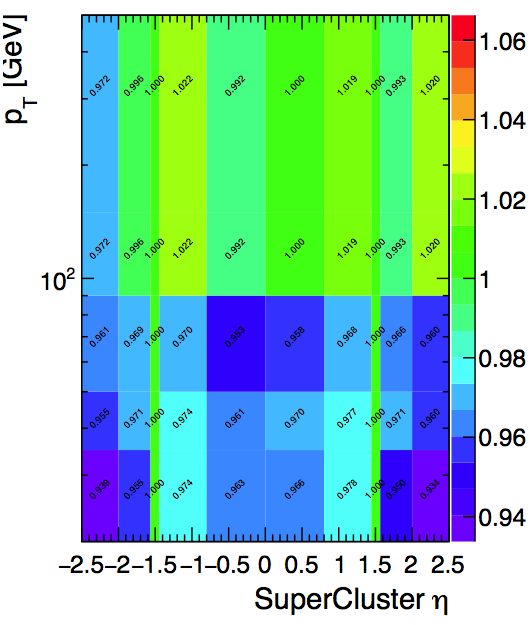
\includegraphics[width=0.49\textwidth]{Figures/EventSelect/scalefactors.png}
    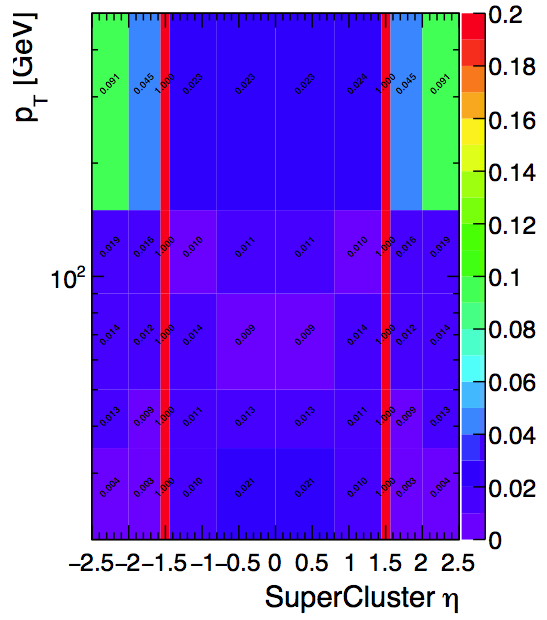
\includegraphics[width=0.49\textwidth]{Figures/EventSelect/sf_errors.png}
    \caption{Calculated scale factors (left) and uncertainties (right)
      in bins of photon \pt and $\eta$.}
    \label{fig:SF}
\end{figure*}

Rather than using the full map of scale factors shown in Figure~\ref{fig:SF},
we compute a weighted average over all photons passing our selection criteria
in each SUSY signal mass point.
The average scale factors and uncertainties are shown in Figure~\ref{fig:SFmap}.

\begin{figure*}[htbp]
    \centering
    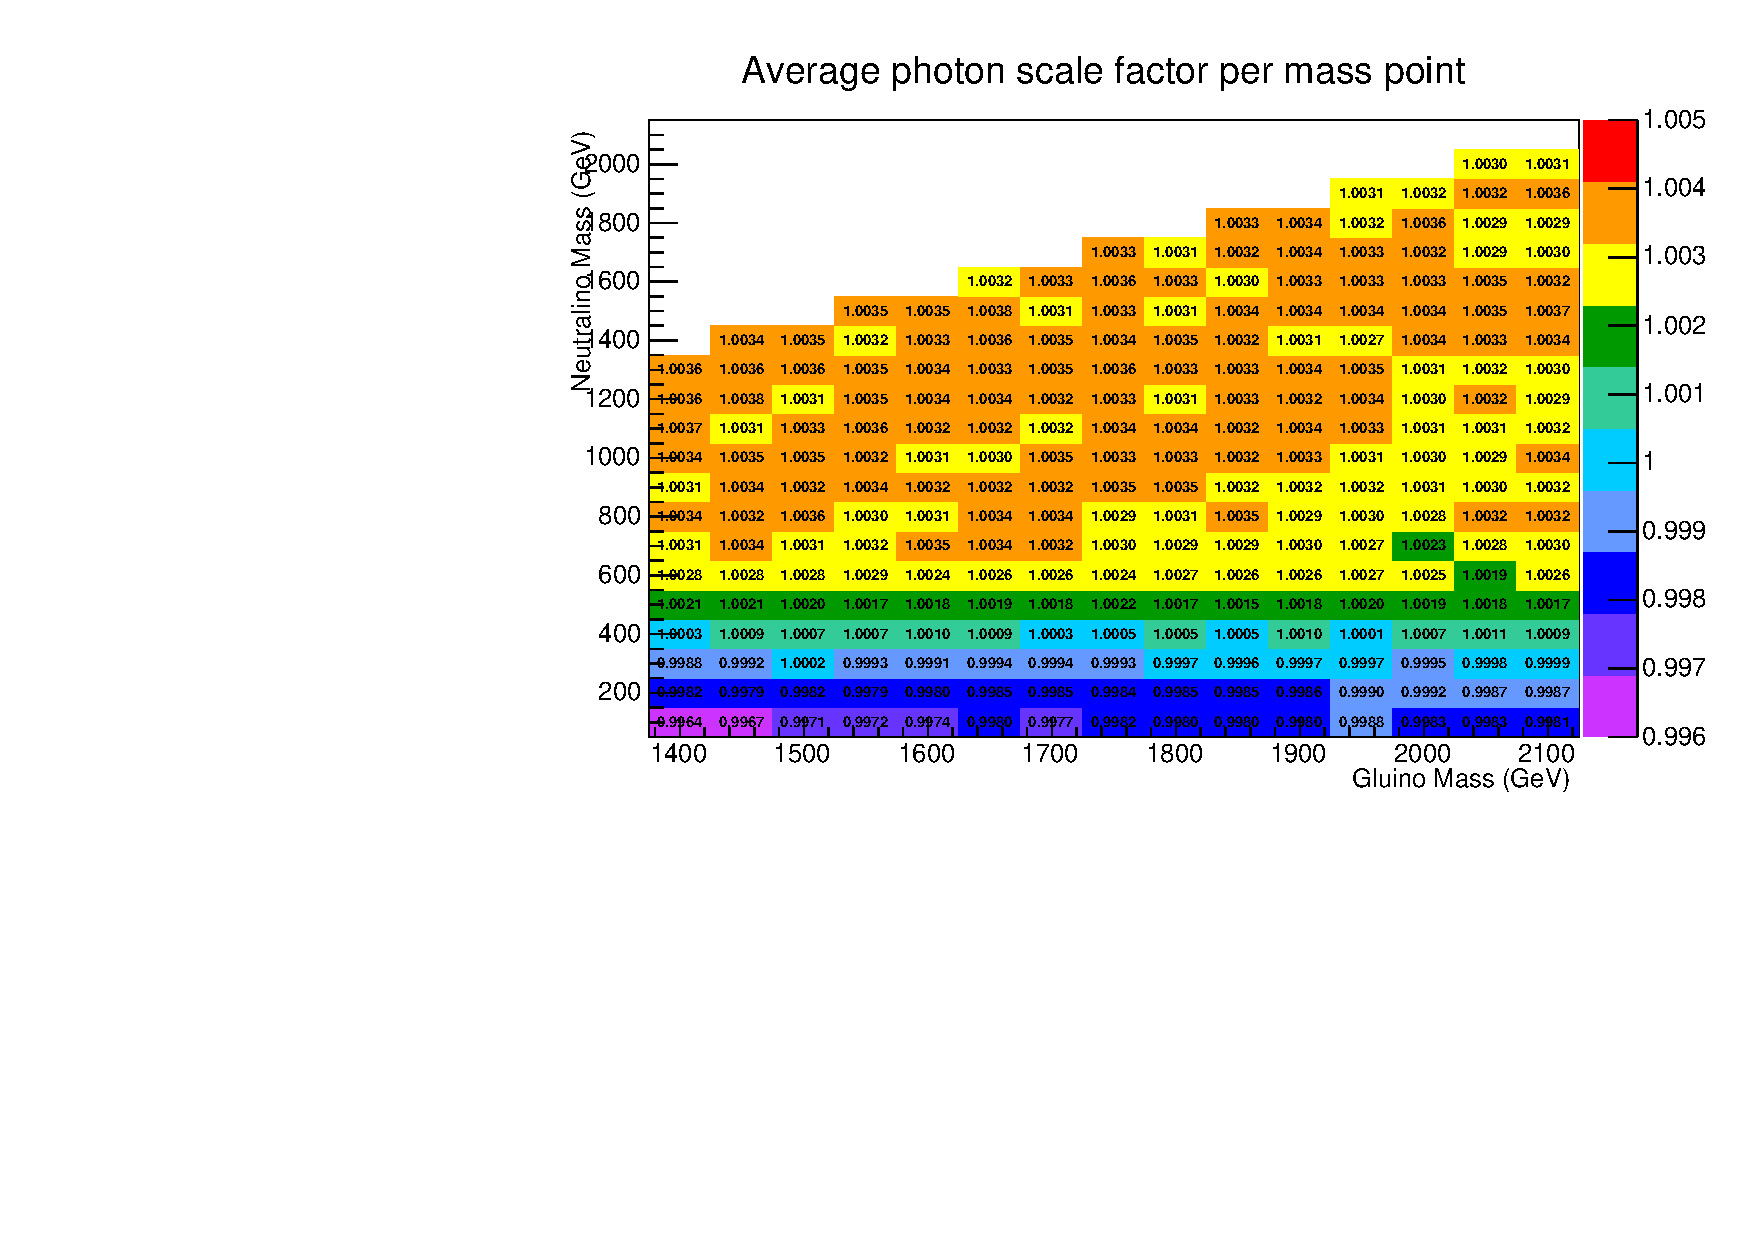
\includegraphics[width=0.8\textwidth]{Figures/EventSelect/sfmap.pdf}
    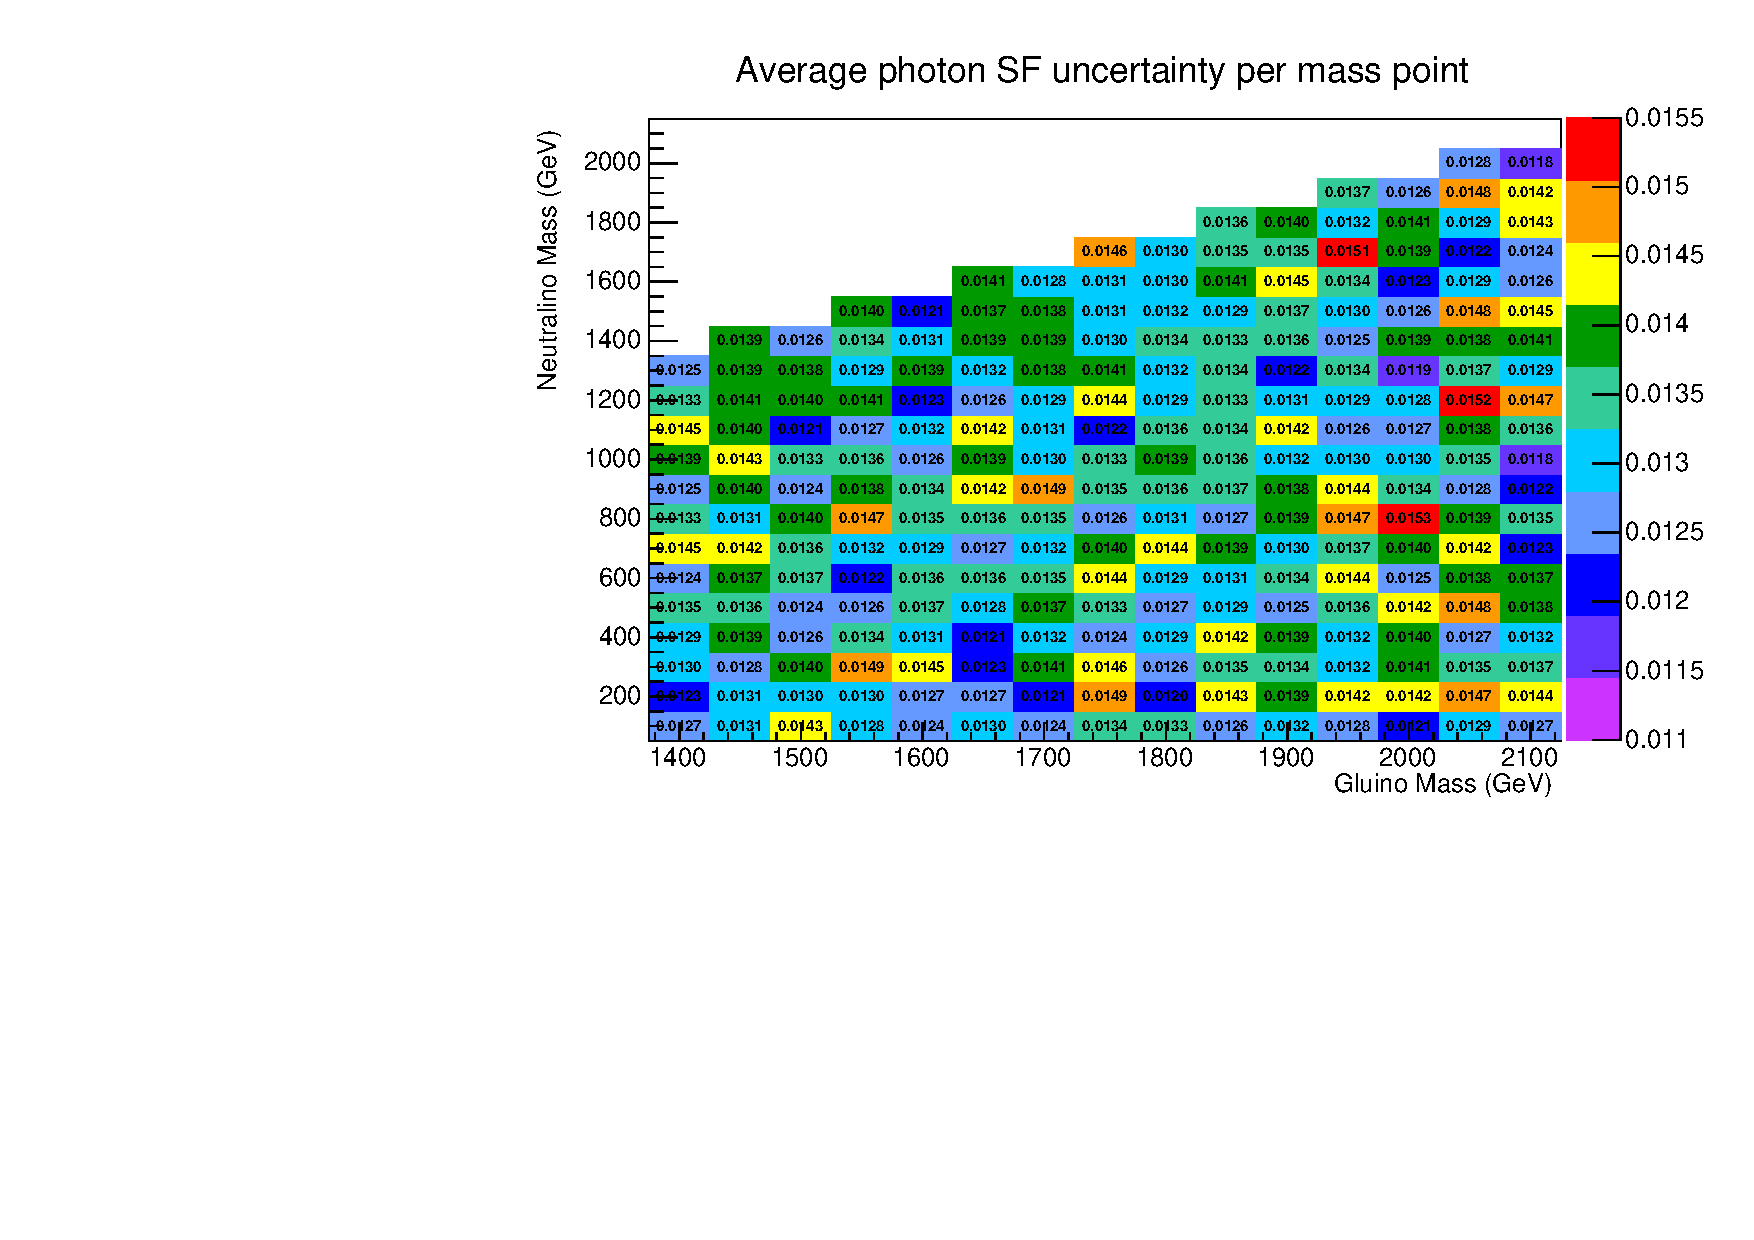
\includegraphics[width=0.8\textwidth]{Figures/EventSelect/sfmap_errors.pdf}
    \caption{Scale factors (top) and uncertainties (bottom)
      averaged over all photons in each bin in the neutralino
      versus gluino mass plane.}
    \label{fig:SFmap}
\end{figure*}

The final value used in the analysis was an average over the mass
points shown in Figure~\ref{fig:SFmap}:
\begin{equation}
  \textrm{Photon Scale Factor} = 1.002\pm0.013
\end{equation}

\subsection{Scale factor for pixel seed veto}
\label{sec:PSV_SF}
Our prescription for photon identification is nearly identical to that for
electron identification, differing only by the presence or absence of a seed
track in the pixel detector. The efficiency of the pixel seed veto
for photons cannot be determined from the tag-and-probe method described above,
and must be obtained from photons in $Z\rightarrow \mu\mu\gamma$
events. Again we use the official scale factor calculated by the
EGM POG:
\begin{equation}
  \textrm{Pixel Seed Veto Scale Factor} = 0.998\pm0.013
\end{equation}

Since our candidate sample requires two photons in the final state,
two factors of both values are used.


\subsection{Scale factor for $R_9$ requirement}
\label{sec:R9SF}
The photon ID used in this analysis differs from the official POG recipe in one aspect: we apply an $R_9 > 0.5$ requirement on top of the medium ID due to the presence of an $R_9$ cut in our analysis trigger. A check was performed to make sure that the $R_9$ requirement does not change the photon scale factors. The results of this study are shown in Figure~\ref{fig:R9SF}. The data/MC scale factors. We therefore choose to simply use the official scale factors described above. 

\begin{figure*}[htbp]
    \centering
    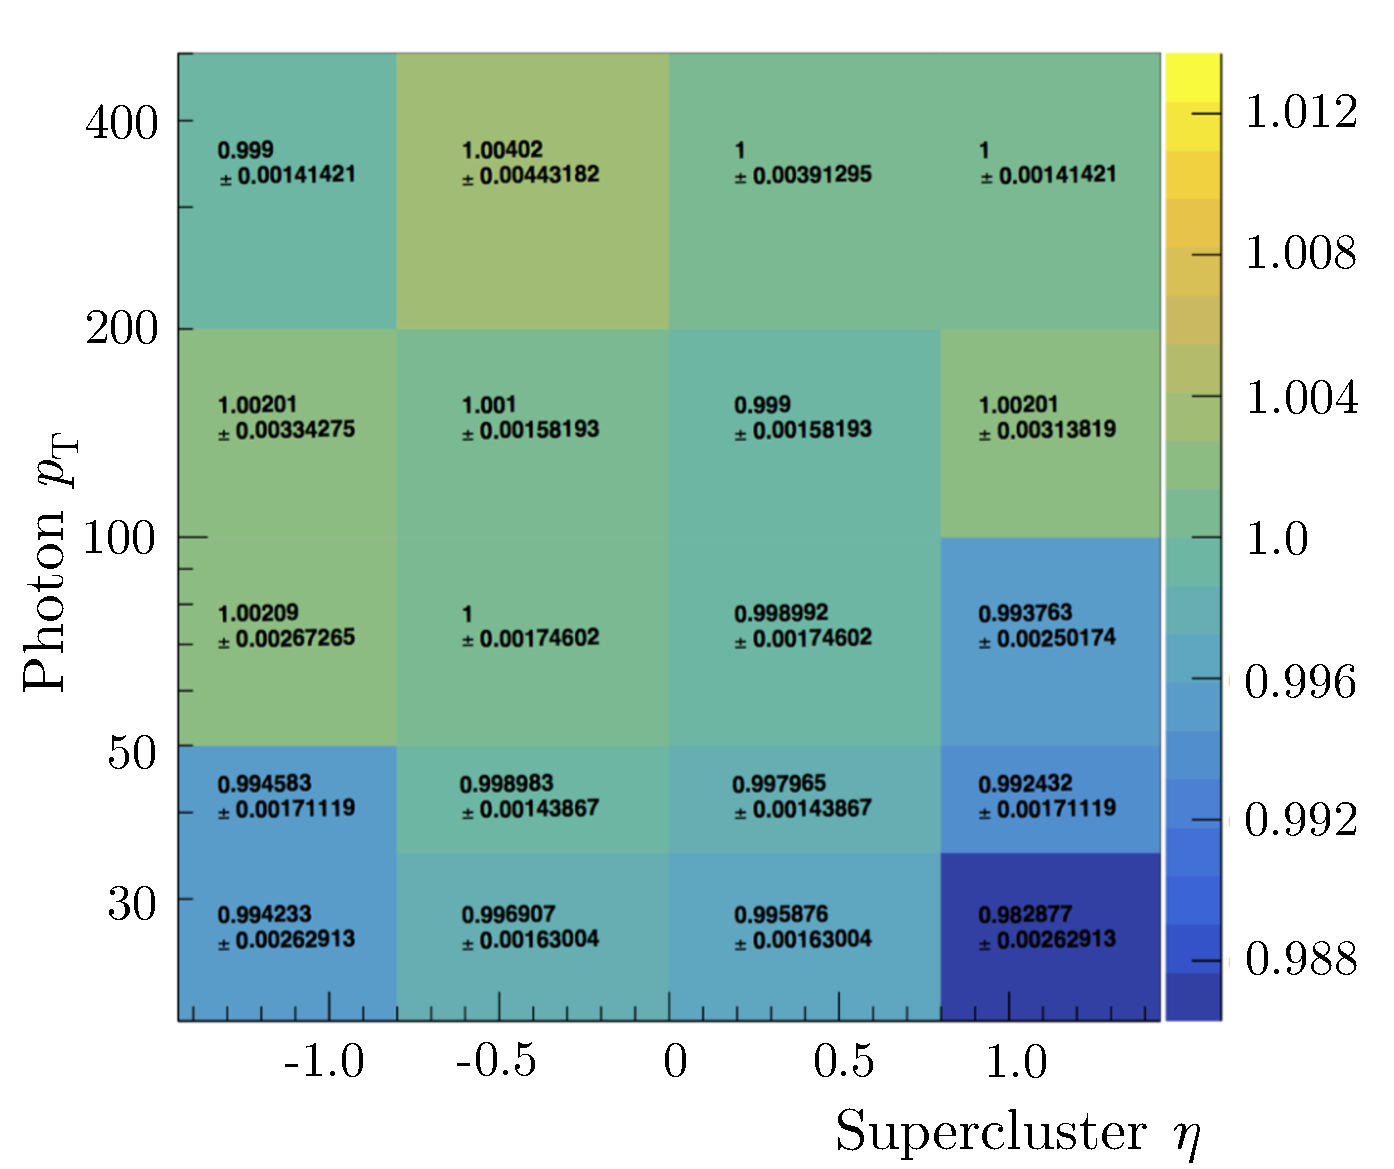
\includegraphics[width=0.9\textwidth]{Figures/EventSelect/R9SF.pdf}
    \caption{Scale factor for applying $R_9 > 0.5$ on top of the cut-based medium photon ID.
    The scale factors are consistent with unity in all bins. Therefore, no additional corrections are applied to
    the scale factors described in Section~\ref{sec:phoSF}.}
    \label{fig:R9SF}
\end{figure*}


